\pdfminorversion=4
\documentclass[aspectratio=169]{beamer}

\mode<presentation>
{\usetheme{metropolis}
%\usecolortheme{spruce}
\usecolortheme{default}
}
%\setbeamertemplate{headline}{}
  %\setbeamercovered{transparent}
  %\expandafter\def\expandafter\insertshorttitle\expandafter{%
  %\insertshorttitle\hfill%
  %\insertframenumber\,/\,\inserttotalframenumber}
%}



\usepackage[T1]{fontenc}
\usepackage[utf8]{inputenc}

\usepackage{times}
\usepackage{amsthm}
\usepackage{graphicx}
\usepackage{subfigure}
\usepackage[mathscr]{eucal}
\usepackage{longtable}
\usepackage[all]{xy}
\usepackage{color}
\usepackage{colortbl}
\usepackage{multirow}
\usepackage{wrapfig}
\usepackage{ragged2e}
\usepackage{epstopdf}
\usepackage{lmodern}


\usepackage{animate}

\usepackage{minted}

\usepackage[]{xcolor}

\definecolor{indigo}{rgb}{0.0, 0.25, 0.42}
\definecolor{arsenic}{rgb}{0.23, 0.27, 0.29}
\definecolor{bluegray}{rgb}{0.4, 0.6, 0.8}
\definecolor{cadet}{rgb}{0.33, 0.41, 0.47}
\definecolor{charcoal}{rgb}{0.21, 0.27, 0.31}
\definecolor{glaucous}{rgb}{0.38, 0.51, 0.71}
\definecolor{airforceblue}{rgb}{0.36, 0.54, 0.66}
\definecolor{darkgreen}{rgb}{0.0, 0.2, 0.13}


\metroset{sectionpage=none, block=fill}

%\setbeamercolor{frametitle}{bg=charcoal,fg=white}
%\setbeamercolor{section in head/foot}{bg=Brown}
%\setbeamercolor{author in head/foot}{bg=Brown}
%\setbeamercolor{date in head/foot}{fg=Brown}

%\setbeamercolor{block title}{bg = airforceblue!80, fg=black}
%\setbeamercolor{block body}{bg=airforceblue!30}

\defbeamertemplate*{frametitle}{}{%
    \leavevmode%
    \hbox to \paperwidth{%
    \begin{beamercolorbox}[wd=\paperwidth,ht=2ex,dp=3pt,left]{frametitle}%
        \ \insertframetitle
    \end{beamercolorbox}}
}




%%%%%%%%%%%% TITLE PAGE %%%%%%%%%%%%%%%%%%
\title[]{\bf CocoTB : python based verification for the RTL projects}
%\author[]{S. Kohani, K. Nishimura, V. Shebalin$^*$}\institute[]{\inst{}
\author{V. Shebalin}
\institute{\inst{}
%Budker Institute of Nuclear Physics\\
{\textit {}}
}
\date[]{December 1,  2022}

%\pgfdeclareimage[height=2.5cm]{mylogo}{Belle-logo.eps}
%%%%%%%%%%%%%%%%%%%%%%%%%%%%%%%%%%%%%%%%%%%



\begin{document}

%%%%%%%%%%%%%%%%%%%%%%%%%%%%%%%%%%%%%%%%%%%%%%%%%%%%
% TITLE PAGE
%%%%%%%%%%%%%%%%%%%%%%%%%%%%%%%%%%%%%%%%%%%%%%%%%%%%
\frame{\titlepage
%\centering \includegraphics[scale=0.3]{figs/uh.png}
}
%%%%%%%%%%%%%%%%%%%%%%%%%%%%%%%%%%%%%%%%%%%%%%%%%%%%

\footnotesize

%%%%%%%%%%%%%%%%%%%%%%%%%%%%%%%%%%%%%%%%%%%%%%%%%%%%
\section*{What Cocotb is?}
%%%%%%%%%%%%%%%%%%%%%%%%%%%%%%%%%%%%%%%%%%%%%%%%%%%%
\begin{frame}{\secname}

  \centering
  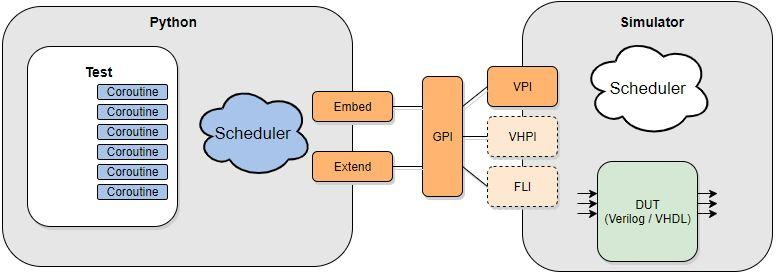
\includegraphics[width=0.9\textwidth]{figs/cocotb_overview.jpg}
  
  \begin{itemize}%[<+->]
    \item \url{https://www.cocotb.org}
    \item A RTL simulator plugin / a python library for writing synchronous logic.
    \item Cocotb is an open source CO-routine-based CO-simulation TestBench
      environment for verifying VHDL and Verilog TRL using Python.
    \item Provides Python interface to control standard RTL simulators (Modelsim/Questa, Cadence, etc.)
    \item Hardware design and verification are different tasks. Verification testbenches are {\bf software} not hardware!


  \end{itemize}
\end{frame}
%%%%%%%%%%%%%%%%%%%%%%%%%%%%%%%%%%%%%%%%%%%%%%%%%%%%

%%%%%%%%%%%%%%%%%%%%%%%%%%%%%%%%%%%%%%%%%%%%%%%%%%%%
\section*{Motivation for python}
%%%%%%%%%%%%%%%%%%%%%%%%%%%%%%%%%%%%%%%%%%%%%%%%%%%%
\begin{frame}{\secname}
  \begin{columns}
    \begin{column}{0.6\textwidth}
      \begin{itemize}
        \item {\bf VHDL} lacks built-in verification tools. 
          OSVVM offers a lot of tools for constrained random testing, 
          functional coverage, message filtering, scoreboards and so on, but it's still VHDL. 
        \item {\bf Verilog/SystemVerilog} -- object oriented language with a lot of verification oriented classes and functions, but it's a pretty difficult language to learn. 
      \end{itemize}
        

      \begin{block}{Why python?}
        \begin{itemize}
          \item Easy to learn
          \item Huge existing ecosystem
          \item Interpreted 
          \item Popular language
          \item Simulation is a software (not hardware), python is good for making software. 
        \end{itemize}
      \end{block}
    \end{column}

    \begin{column}{0.5\textwidth}
      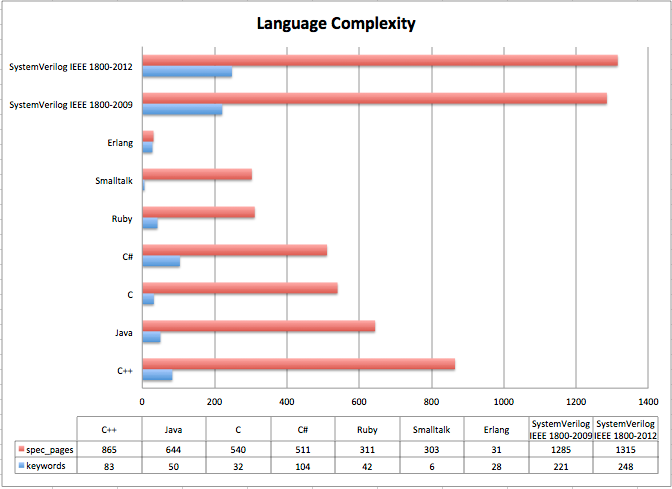
\includegraphics[width=1.0\textwidth]{figs/lang_coplexity.png}
    \end{column}
  \end{columns}
  	
\end{frame}
%%%%%%%%%%%%%%%%%%%%%%%%%%%%%%%%%%%%%%%%%%%%%%%%%%%%

%%%%%%%%%%%%%%%%%%%%%%%%%%%%%%%%%%%%%%%%%%%%%%%%%%%%
\section*{Some of HEP specifics}
%%%%%%%%%%%%%%%%%%%%%%%%%%%%%%%%%%%%%%%%%%%%%%%%%%%%
\begin{frame}{\secname}
  \begin{itemize}
    \item Physics group -- they know what kind of output they need from the electronics, know physics, 
      don't know technical details, don't know HDL, most likely know python
    \item Electronics group -- they know all details of the electronics, don't have proficiency in data analysis
  \end{itemize}
   \begin{columns}
     \begin{column}{0.5\textwidth}
       \begin{block}{Physics group}
           \begin{itemize}
           \item Know what they need the electronics for.
           \item Don't know the details of the digital design. 
           \item Have the realistic data for the electronics input signals 
             (MC simulation, experimental data samples).
           \item Have the tools to analyze the data electronics should provide.
           \item Most likely know python.
           \end{itemize}
         
       \end{block}
     \end{column}
     \begin{column}{0.5\textwidth}
       \begin{block}{Electronics group}
         \begin{itemize}
           \item Probably don't know all the aspects of the electronics application. 
           \item Know everything about details of the logic implementation. 
           \item Have their oscilloscopes and pulse generators for the basic testing. 
           \item Most likely know python. 
         \end{itemize}
         
       \end{block}
       
     \end{column}
   \end{columns}
    
   There are  verification engineers in big companies and big experiments, but smaller groups usually have very limited manpower. Cocotb makes it possible to bring more people into firmware verification: students, software experts, physicists. 

\end{frame}
%%%%%%%%%%%%%%%%%%%%%%%%%%%%%%%%%%%%%%%%%%%%%%%%%%%%


%%%%%%%%%%%%%%%%%%%%%%%%%%%%%%%%%%%%%%%%%%%%%%%%%%%%
\section*{Cocotb workflow}
%%%%%%%%%%%%%%%%%%%%%%%%%%%%%%%%%%%%%%%%%%%%%%%%%%%%
\begin{frame}{\secname}
  \begin{columns}[c]
    \begin{column}{0.5\textwidth}
      \begin{block}{Cocotb main features}
        \begin{itemize} %[<+->]
          \item { Design under test (DUT) runs in a standard simulator. }
          \item { cocotb provides interface between simulator and Python (compiled C++ library called GPI).}
          \item { Simulator is controlled by VPI, VHPI, or FLI interfaces.}
          \item { Python testbench allows to: access DUT hierarchy, wait for simulator time to advance, trigger on different conditions}
        \end{itemize}
      \end{block}
      
    \end{column}
    \begin{column}{0.55\textwidth}
      \vspace*{1mm}
      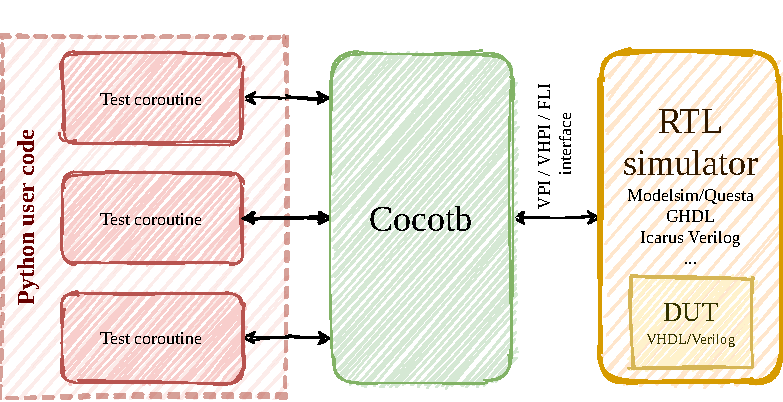
\includegraphics[width=1.0\textwidth]{figs/cocotb_sim.pdf}\\
      \begin{exampleblock}{Python basis }
        \begin{itemize}
          \item {\bf async functions} -- not called directly, but {\it awaited} instead
          \item {\bf coroutines} -- cooperative multitasking routines. 
          \item {\bf decorators} -- some kind of a wrapper function 
         \end{itemize}
          Prior to python 3.5 cocotb used generators/yield to emulate concurrent processing. 
         
       \end{exampleblock}
    \end{column}
  \end{columns}
   
\end{frame}
%%%%%%%%%%%%%%%%%%%%%%%%%%%%%%%%%%%%%%%%%%%%%%%%%%%%


%%%%%%%%%%%%%%%%%%%%%%%%%%%%%%%%%%%%%%%%%%%%%%%%%%%%
\section*{Cocotb basic example}
%%%%%%%%%%%%%%%%%%%%%%%%%%%%%%%%%%%%%%%%%%%%%%%%%%%%
\begin{frame}[fragile]{\secname}

  \begin{columns}[t]
    \scriptsize
    \begin{column}{0.4\textwidth}
      \centering 
      {\bf dff.vhd}
      
      \begin{minted}{vhdl}
        library ieee;
        use ieee.std_logic_1164.all;
         
        entity dff is
        port(
          clk: in std_logic;
          d: in std_logic;
          q: out std_logic);
        end dff;
         
        architecture behavioral of dff is
        begin
          process (clk) begin
            if rising_edge(clk) then
              q <= d;
            end if;
          end process;
        end behavioral;

      \end{minted}
      %\pause
      
    \end{column}
    \begin{column}{0.7\textwidth}
      \centering 
      {\bf test$\rm\_$dff.py}
        \begin{minted}{python}
          import cocotb   
          from cocotb.clock import Clock
          from cocotb.triggers import RisingEdge
                          
          @cocotb.test() 
          async def test_dff(dut):
              # Create a 10us period clock on port clk
              clock = Clock(dut.clk, 10, units="us")  
              # Start the clock
              cocotb.start_soon(clock.start())  
                          
              dut.d.value = 0  
              await RisingEdge(dut.clk)  
              dut.d.value = 1  
              await RisingEdge(dut.clk)
              assert dut.q.value == 1, f"Error!"

        \end{minted}
        \centering {\color{red} \it Compare it to the VHDL testbench!}
      
    \end{column}

  \end{columns}


  {\color{blue} \url{https://github.com/vsheb/cocotb_practice}} -- my non-professional examples I did for practice
\end{frame}
%%%%%%%%%%%%%%%%%%%%%%%%%%%%%%%%%%%%%%%%%%%%%%%%%%%%


%%%%%%%%%%%%%%%%%%%%%%%%%%%%%%%%%%%%%%%%%%%%%%%%%%%%
\section*{Makefiles}
%%%%%%%%%%%%%%%%%%%%%%%%%%%%%%%%%%%%%%%%%%%%%%%%%%%%
\begin{frame}[fragile]{\secname}
  
  \begin{block}{Minimal makefile example}
    \begin{minted}{make}
      VHDL_SOURCES = dff.vhd
      TOPLEVEL := dff
      MODULE   := test_dff

      include $(shell cocotb-config --makefiles)/Makefile.sim
    \end{minted}

    \begin{block}{Run it}
      \begin{minted}{bash}
        pip3 install cocotb # install cocotb if you haven't done it yet
        make # run cocotb
      \end{minted}
    \end{block}

    \begin{block}{Output}
    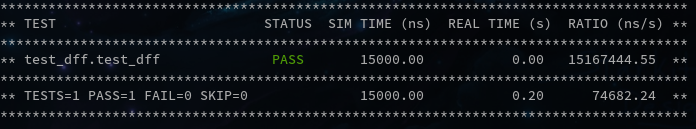
\includegraphics[width=1.0\textwidth]{figs/cocotb_dff.png}
    \end{block}
    
    
  \end{block}
    
\end{frame}
%%%%%%%%%%%%%%%%%%%%%%%%%%%%%%%%%%%%%%%%%%%%%%%%%%%%

%%%%%%%%%%%%%%%%%%%%%%%%%%%%%%%%%%%%%%%%%%%%%%%%%%%%%
\section*{View the waveform}
%%%%%%%%%%%%%%%%%%%%%%%%%%%%%%%%%%%%%%%%%%%%%%%%%%%%%
\begin{frame}[fragile]{\secname}
  \begin{block}{Makefile}
    \begin{minted}{make}
      VHDL_SOURCES = dff.vhd
      TOPLEVEL := dff
      MODULE   := test_dff
      ## Save waveforms
      WAVES    := 1

      include $(shell cocotb-config --makefiles)/Makefile.sim
    \end{minted}

    \begin{block}{View waveform \tiny (you can use any supported simulator, not only {\it gtkwave}, obviously)}
    \begin{minted}{bash}
      gtkwave dff.vcd 
    \end{minted}
    \end{block}
  \end{block}

    
    
\end{frame}
%%%%%%%%%%%%%%%%%%%%%%%%%%%%%%%%%%%%%%%%%%%%%%%%%%%%%


%%%%%%%%%%%%%%%%%%%%%%%%%%%%%%%%%%%%%%%%%%%%%%%%%%%%
\section*{cocotb-test}
%%%%%%%%%%%%%%%%%%%%%%%%%%%%%%%%%%%%%%%%%%%%%%%%%%%%
\begin{frame}[fragile]{\secname}
  \begin{exampleblock}{Makefile pros and cons}
    \begin{itemize}
      \item \color{darkgreen} Allows integration of verification into the building process.
      \item \color{red} An extra file to take care of.
    \end{itemize}
   
  \end{exampleblock}
  
  As an alternative to makefiles there is the cocotb-test package which makes it possible to run cocotb tests as a standalone program.\\
  \color{blue}
  \url{https://github.com/themperek/cocotb-test}
  \color{black}

  {\bf cocotb-test} provides standard python unit testing capabilities for cocotb
  \begin{itemize}
    \item allow the look and feel of Python unit testing (see \url{pytest.org})
    \item remove the need for Makefiles (includes Makefile compatibility mode)
    \item allow easy customization of simulation flow
    \item allow to use pytest-xdist or pytest-parallel for parallel runs
  \end{itemize}

  \begin{block}{Installation}
  \begin{minted}[]{bash}
  pip install cocotb-test
  \end{minted}
  \end{block}


    
\end{frame}
%%%%%%%%%%%%%%%%%%%%%%%%%%%%%%%%%%%%%%%%%%%%%%%%%%%%

%%%%%%%%%%%%%%%%%%%%%%%%%%%%%%%%%%%%%%%%%%%%%%%%%%%%
\section*{cocotb-test example}
%%%%%%%%%%%%%%%%%%%%%%%%%%%%%%%%%%%%%%%%%%%%%%%%%%%%
\begin{frame}[fragile]{\secname}
    \begin{block}{import cocotb-test}
    \begin{minted}{python}
  from cocotb_test.simulator import run
    \end{minted}
\end{block}


\begin{block}{Run the test without invoking make}
  \begin{minted}{python}
def run_test_dff():
  run(
    vhdl_sources  = ['dff.vhd'], # the list of vhdl sources to be included
    toplevel      = 'dff',       # DUT
    module        = 'test_dff1', # python module which contains coroutines to run
    toplevel_lang = 'vhdl',
    sim_args      = ['--vcd=dff.vcd'], # this one is specific to ghdl simulator 
    waves         = 1)
if __name__ == "__main__" :
  run_test_dff()

  \end{minted}
\end{block}
  Among other things cocotb-test allows for running parametrized tests.
\end{frame}
%%%%%%%%%%%%%%%%%%%%%%%%%%%%%%%%%%%%%%%%%%%%%%%%%%%%


%%%%%%%%%%%%%%%%%%%%%%%%%%%%%%%%%%%%%%%%%%%%%%%%%%%%
\section*{Accessing the hierarchy}
%%%%%%%%%%%%%%%%%%%%%%%%%%%%%%%%%%%%%%%%%%%%%%%%%%%%
\begin{frame}[fragile]{\secname}
  Cocotb makes it possible to access the internal signal by it's hierarchy using the simulator interface 
  even if the language (i.e. VHDL-93) doesn't allow to do so.
  \begin{block}{Usage examples}
  \begin{minted}{python}
# access the current value of the signal of interest
val = int(dut.module.submodule.signal.value)
# change the current value of the signal
dut.module.submodule.signal.value = 1
# force a handle to a given value 
dut.module.submodule.signal.value = Force(1)  
# make a handle keep its current value
dut.module.submodule.signal.value = Freeze() 
# stop the effects of a previously applied force/freeze action
dut.module.submodule.signal.value = Release() 
  \end{minted}
  \end{block}
Hierarchy access to the internal signals gives a very flexible way to simulate single event upsets.
    
\end{frame}
%%%%%%%%%%%%%%%%%%%%%%%%%%%%%%%%%%%%%%%%%%%%%%%%%%%%

%%%%%%%%%%%%%%%%%%%%%%%%%%%%%%%%%%%%%%%%%%%%%%%%%%%%
\section*{Coroutines}
%%%%%%%%%%%%%%%%%%%%%%%%%%%%%%%%%%%%%%%%%%%%%%%%%%%%
\begin{frame}[fragile]{\secname}
  \scriptsize
  \begin{itemize}
    \item Any function which imply advancing of the simulation time must be {\bf coroutine}.
    \item Cocotb coroutines emulate synchronous {\it \bf process}(VHDL) or {\it \bf always}(Verilog) blocks.
    \item Can run in parallel. 
    \item A key thing to create complex testbenches : different coroutines running in parallel may serve as {\bf drivers} and {\bf monitors}.
  \end{itemize}

  \vspace*{-2mm}
  \begin{columns}
    \begin{column}{0.5\textwidth}

  \begin{minted}[linenos,frame=lines]{python}
@coroutine
async def dff_driver(dut):
  dut.d.value = 0
  for _ in range(100) : 
    await RisingEdge(dut.clk)
    dut.d.value = 1
    await RisingEdge(dut.clk)
    dut.d.value = 0
    await ClockCycles(dut.clk, 10)
  \end{minted}
      
    \end{column}

    \begin{column}{0.5\textwidth}

  \begin{minted}[linenos,frame=lines]{python}
@coroutine
async def dff_monitor(dut):
  while True:
    await RisingEdge(dut.clk)
    if dut.d.value == 1 :
      await RisingEdge(dut.clk)
      assert dut.q.value == 1, f"Error!"
  \end{minted}
    \end{column}
  \end{columns}

 In older examples you may see {\it @cocotb.coroutine} decorator which is deprecated, also {\it yield} keyword has been replaced with {\it await} starting from version 1.4.0 (2020).

\end{frame}
%%%%%%%%%%%%%%%%%%%%%%%%%%%%%%%%%%%%%%%%%%%%%%%%%%%%

%%%%%%%%%%%%%%%%%%%%%%%%%%%%%%%%%%%%%%%%%%%%%%%%%%%%
\section*{Starting coroutines}
%%%%%%%%%%%%%%%%%%%%%%%%%%%%%%%%%%%%%%%%%%%%%%%%%%%%
\begin{frame}[fragile]{\secname}

  \begin{columns}
    \begin{column}{0.5\textwidth}
      
  \begin{minted}[frame=lines,framesep=2mm]{python}
@cocotb.test()
async def test_dff(dut):
  # start clock
  clk = Clock(dut.clk, 10, units="ns") 
  cocotb.start_soon(clk.start())

  # start monitoring 
  mon = cocotb.start_soon(dff_monitor(dut))
  # start driver
  drv = cocotb.start_soon(dff_driver(dut))
  
  # wait the driver coroutine to finish
  await Join(drv)
  \end{minted}
    \end{column}
    \begin{column}{0.5\textwidth}
      \begin{block}{Methods to start a coroutine}
         \begin{itemize}
           \item {\bf fork()} -- (deprecated) schedules and executes the new coroutine immediately, no other pending tasks are run. 
           \item {\bf start()} -- schedules the new coroutine to be executed concurrently, then yields control to allow the new task (and any other pending tasks) to run, before resuming the calling task.
            \item {\bf start$\_$soon()} -- schedules the new coroutine for future execution, after the calling task yields control.
         \end{itemize}
      \end{block}
      
    \end{column}
  \end{columns}
    
\end{frame}
%%%%%%%%%%%%%%%%%%%%%%%%%%%%%%%%%%%%%%%%%%%%%%%%%%%%

%%%%%%%%%%%%%%%%%%%%%%%%%%%%%%%%%%%%%%%%%%%%%%%%%%%%
\section*{Triggers}
%%%%%%%%%%%%%%%%%%%%%%%%%%%%%%%%%%%%%%%%%%%%%%%%%%%%
\begin{frame}{\secname}
  Triggers are used to indicate when the cocotb scheduler should resume coroutine execution. In other words the execution of the python code has been stopped and simulation time advances until trigger condition is met. To use a trigger, a coroutine should {\bf await} it. 

  \centering
  \begin{tabular}{l|l}
    Edge(signal) & Fires on any value change of signal. \\ \hline
    RisingEdge(signal) & Fires on the rising edge of signal.\\ \hline
    FallingEdge(signal) & Fires on the falling edge of signal. \\ \hline
    ClockCycles(signal,num) & Fires after {\it num} transactions of signal from 0 to 1.\\ \hline
    Timer(time) & Fires after the specific simulation time period elapsed. \\ \hline\hline
    Join(coroutine) & Fires when a task completes. \\ \hline
    Combine(*triggers) & Fires when all triggers have fired. \\ \hline
    First(*triggers)   & Fires when the first trigger fires. \\ \hline
    Event()            & Event to permit synchronization between coroutines.
  \end{tabular}
    
\end{frame}
%%%%%%%%%%%%%%%%%%%%%%%%%%%%%%%%%%%%%%%%%%%%%%%%%%%%

%%%%%%%%%%%%%%%%%%%%%%%%%%%%%%%%%%%%%%%%%%%%%%%%%%%%
\section*{Communication between coroutines}
%%%%%%%%%%%%%%%%%%%%%%%%%%%%%%%%%%%%%%%%%%%%%%%%%%%%
\begin{frame}[fragile]{\secname}
  There are two basic approaches to pass the information between coroutines: 
  \begin{itemize}
    \item Using the Event() trigger, the data in transferred by setting event.data.
    \item Using the python {\bf classes}. Class methods may be cocotb coroutines and
      at the same time have access to the class data objects. 
  \end{itemize}
  
    
\end{frame}
%%%%%%%%%%%%%%%%%%%%%%%%%%%%%%%%%%%%%%%%%%%%%%%%%%%%

%%%%%%%%%%%%%%%%%%%%%%%%%%%%%%%%%%%%%%%%%%%%%%%%%%%%
\section*{Classes as testbenches}
%%%%%%%%%%%%%%%%%%%%%%%%%%%%%%%%%%%%%%%%%%%%%%%%%%%%
\begin{frame}[fragile]{\secname}

  \begin{minted}[linenos,numbersep=5pt,frame=lines,framesep=2mm]{python}
import cocotb
from cocotb.triggers import RisingEdge, FallingEdge

class TestBench : 
  def __init__(self,dut):
  self.dut = dut
  self.expected_data = [] # this will be accessible by both monitor and driver

  @coroutine
  async def drive(self,dut):
    # drive DUT inputs with randomized/preset values
    # set the data expected at output based on what we set at input
  
  @coroutine
  async def monitor(self,dut):
    # monitor DUT outputs and compare to the expected values
    # compare actual outputs to the expected ones

    \end{minted}
    
\end{frame}
%%%%%%%%%%%%%%%%%%%%%%%%%%%%%%%%%%%%%%%%%%%%%%%%%%%%

%%%%%%%%%%%%%%%%%%%%%%%%%%%%%%%%%%%%%%%%%%%%%%%%%%%%
\section*{Cocotb extensions}
%%%%%%%%%%%%%%%%%%%%%%%%%%%%%%%%%%%%%%%%%%%%%%%%%%%%
\begin{frame}{\secname}
  \href{https://github.com/cocotb/cocotb-bus}{\color{blue}cocotb-bus} -- 
  testbenching tools and reusable bus interfaces\\
  \href{https://github.com/mciepluc/cocotb-coverage}{\color{blue}cocotb-coverage} -- 
  an extension for functional coverage and constrained randomization.\\
  A complete list of extension modules may be found 
\href{https://github.com/cocotb/cocotb/wiki/Further-Resources\#extension-modules-cocotbext}{\color{blue}here}.

    \centering
    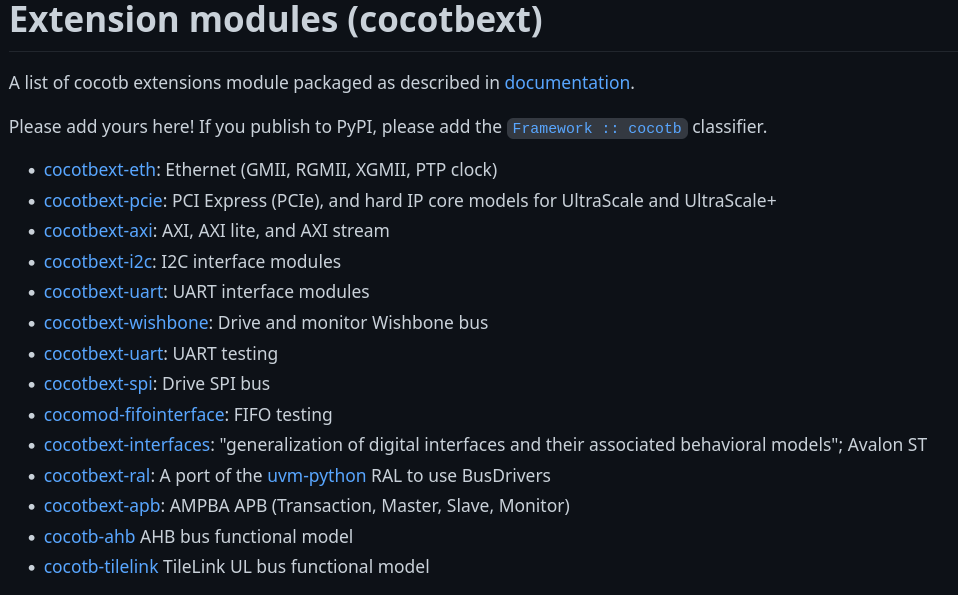
\includegraphics[width=0.7\textwidth]{figs/cocotb_ext_github.png}
    
\end{frame}
%%%%%%%%%%%%%%%%%%%%%%%%%%%%%%%%%%%%%%%%%%%%%%%%%%%%



%%%%%%%%%%%%%%%%%%%%%%%%%%%%%%%%%%%%%%%%%%%%%%%%%%%%
\section*{Integration with other tools}
%%%%%%%%%%%%%%%%%%%%%%%%%%%%%%%%%%%%%%%%%%%%%%%%%%%%
\begin{frame}{\secname}

  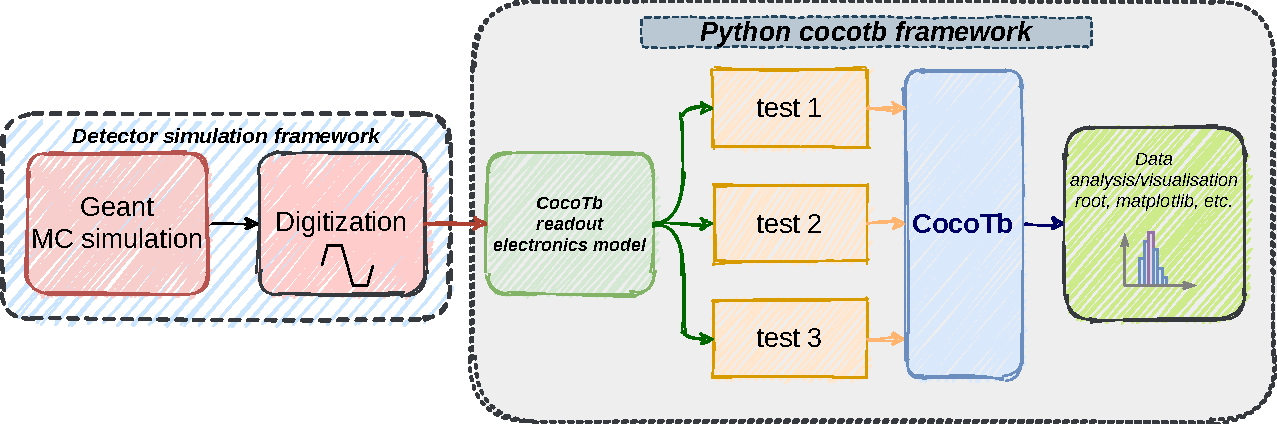
\includegraphics[width=1.0\textwidth]{figs/cocotb_integration.pdf}

  \vspace*{-3mm}
  \begin{itemize}
    \item Cocotb testbenches are python scripts, so they can use all the power of python. 
    \item It's much easier to make functional models of the devices 
      (e.g. ADC, DRS4, custom chips, etc.) in python than in HDL. 
    \item Rapid prototyping of logic for hardware components which don't exist yet. 
    \item Visualization and data analysis with matplotlib, CERN Root or other tools. 
  \end{itemize}
  
   \centering
   (to be continued...)
\end{frame}
%%%%%%%%%%%%%%%%%%%%%%%%%%%%%%%%%%%%%%%%%%%%%%%%%%%%

%%%%%%%%%%%%%%%%%%%%%%%%%%%%%%%%%%%%%%%%%%%%%%%%%%%%
\section*{Further reading}
%%%%%%%%%%%%%%%%%%%%%%%%%%%%%%%%%%%%%%%%%%%%%%%%%%%%
\begin{frame}[fragile]{\secname}
  The cocotb community collects all materials on cocotb available on internet: 
  {\color{blue} https://github.com/cocotb/cocotb/wiki/Further-Resources} \\
  There is a complete list of extension modules, lots of links to custom libraries and examples, youtube lectures and streams, etc. 

   \begin{exampleblock}{More topics might be covered}
     \begin{itemize}
      \item More complex examples from real projects. 
      \item Basics of verification theory: constrained random testing, functional coverage, etc. 
      \item Testbenching tools for reusable bus interfaces : cocotb-bus. 
      \item Other open-source tools for FPGA development and verification: ghdl, Yosys, X-Ray project, OSVWM.
     \end{itemize}
     
   \end{exampleblock}
    
\end{frame}
%%%%%%%%%%%%%%%%%%%%%%%%%%%%%%%%%%%%%%%%%%%%%%%%%%%%



\end{document}




